%
% $RCSfile: container.tex,v $
%
% Copyright (C) 2002-2008. Christian Heller.
%
% Permission is granted to copy, distribute and/or modify this document
% under the terms of the GNU Free Documentation License, Version 1.1 or
% any later version published by the Free Software Foundation; with no
% Invariant Sections, with no Front-Cover Texts and with no Back-Cover
% Texts. A copy of the license is included in the section entitled
% "GNU Free Documentation License".
%
% http://www.cybop.net
% - Cybernetics Oriented Programming -
%
% http://www.resmedicinae.org
% - Information in Medicine -
%
% Version: $Revision: 1.1 $ $Date: 2008-08-19 20:41:06 $ $Author: christian $
% Authors: Christian Heller <christian.heller@tuxtax.de>
%

\subsubsection{Container}
\label{container_heading}
\index{Container}
\index{Primitive Type}
\index{Java Container Framework}
\index{Collection}
\index{Map}
\index{Tree}
\index{Standard Template Library}
\index{STL}
\index{Sequence}
\index{Associative Container}

An object that got created through instantiating a class represents an
allocated area in a computer's memory which needs to be referenced in order to
be able to work with it, and to finally destroy it. The size of that area may
change \emph{dynamically}, depending on how the properties of the object are
manipulated. Primitive types like \emph{integer} or \emph{double} also reserve
memory space, only that the size of that space is \emph{not} dynamic; it is
pre-defined by the programming language, for each type. All
\emph{Structured- and Procedural Programming} (SPP) languages and some
\emph{Object Oriented Programming} (OOP) languages, like Java, offer standard
primitive types.

\begin{figure}[ht]
    \begin{center}
        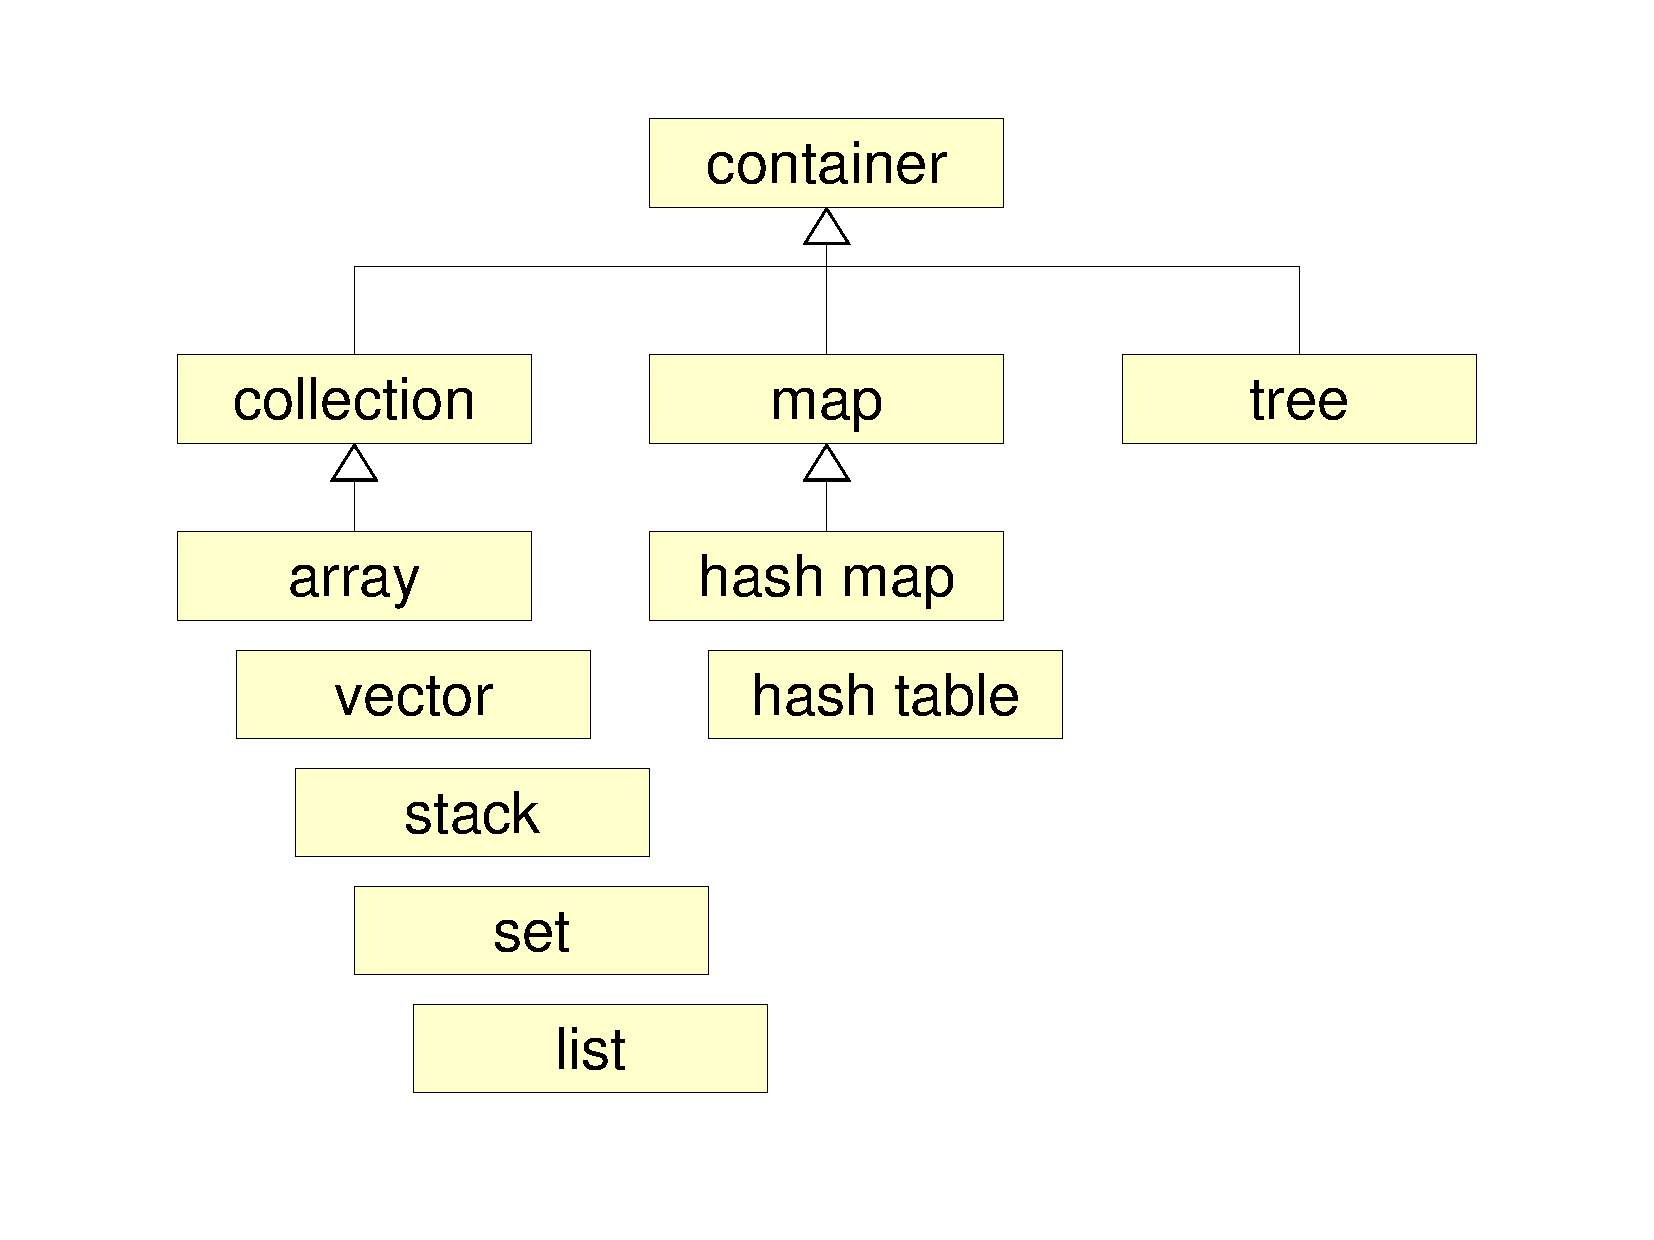
\includegraphics[scale=0.3,angle=-90]{graphic/container.pdf}
        \caption{Java Container Framework Systematics}
        \label{container_figure}
    \end{center}
\end{figure}

One way to store references to more than one dynamic element in memory, or
primitive data, is a \emph{Container}. Modern programming languages offer many
different kinds of containers. Figure \ref{container_figure} shows a
systematics of the Java container framework \cite{java}, as example, which gets
briefly introduced in the following paragraphs. Its main categories of
systematisation are \emph{Collection}, \emph{Map} and \emph{Tree}.

A similar library of container classes, algorithms and iterators exists for the
C++ programming language. It is called \emph{Standard Template Library} (STL)
\cite{stl} and it talks of \emph{Sequence} and \emph{Associative Container},
where Java says \emph{Collection} and \emph{Map}.

%
% $RCSfile: collection.tex,v $
%
% Copyright (C) 2002-2008. Christian Heller.
%
% Permission is granted to copy, distribute and/or modify this document
% under the terms of the GNU Free Documentation License, Version 1.1 or
% any later version published by the Free Software Foundation; with no
% Invariant Sections, with no Front-Cover Texts and with no Back-Cover
% Texts. A copy of the license is included in the section entitled
% "GNU Free Documentation License".
%
% http://www.cybop.net
% - Cybernetics Oriented Programming -
%
% http://www.resmedicinae.org
% - Information in Medicine -
%
% Version: $Revision: 1.1 $ $Date: 2008-08-19 20:41:05 $ $Author: christian $
% Authors: Christian Heller <christian.heller@tuxtax.de>
%

\paragraph{Collection}
\label{collection_heading}
\index{Collection}
\index{Array}
\index{Allocated Area}
\index{Random Access Memory}
\index{RAM}
\index{Vector}
\index{Stack}
\index{Last-In-First-Out}
\index{LIFO}
\index{Set}
\index{List}
\index{Duplicate Element}
\index{Ordered Collection}
\index{Sequence}
\index{Enumeration}
\index{nextElement Method}
\index{Java Development Kit}
\index{JDK}
\index{Iterator}

The \emph{Array} is the most basic form of a container. It represents an allocated
area in the computer's \emph{Random Access Memory} (RAM). A \emph{Vector}
implements a dynamically growable array of objects. The \emph{Stack} class extends
the vector class and represents a \emph{Last-In-First-Out} (LIFO) stack of objects.
A collection that contains no duplicate elements is called a \emph{Set}. Unlike
sets, \emph{Lists} typically allow duplicate elements. Synonyms for list are
\emph{Ordered Collection} and \emph{Sequence}.

Objects that can generate a series of elements, one at a time, implement the
\emph{Enumeration} interface. Successive calls to the \emph{nextElement} method
return successive elements of such a series. In recent releases of the
\emph{Java Development Kit} (JDK) \cite{java}, \emph{Iterator} takes the place
of enumeration, in the collections framework. An iterator over a collection
differs from an enumeration in that it allows the caller to remove elements,
with well-defined semantics, from the underlying collection during an iteration.

%
% $RCSfile: map.tex,v $
%
% Copyright (C) 2002-2008. Christian Heller.
%
% Permission is granted to copy, distribute and/or modify this document
% under the terms of the GNU Free Documentation License, Version 1.1 or
% any later version published by the Free Software Foundation; with no
% Invariant Sections, with no Front-Cover Texts and with no Back-Cover
% Texts. A copy of the license is included in the section entitled
% "GNU Free Documentation License".
%
% http://www.cybop.net
% - Cybernetics Oriented Programming -
%
% http://www.resmedicinae.org
% - Information in Medicine -
%
% Version: $Revision: 1.1 $ $Date: 2008-08-19 20:41:07 $ $Author: christian $
% Authors: Christian Heller <christian.heller@tuxtax.de>
%

\paragraph{Map}
\label{map_heading}
\index{Map}
\index{Dictionary}
\index{Table}
\index{Key-Value-Pair}
\index{Duplicate Key}
\index{Hash Map}
\index{Hash Table}
\index{Null Value}
\index{Null Key}

A \emph{Map} (also called \emph{Dictionary} or \emph{Table}) is an object that
maps \emph{Keys} to \emph{Values}. It cannot contain duplicate keys; each key
can map to at most one value. Java offers two kinds of a map: \emph{Hash Map}
and \emph{Hash Table}. The former is roughly equivalent to the latter, except
that it permits null values and the null key \cite{java, gumbel}.

%
% $RCSfile: tree.tex,v $
%
% Copyright (C) 2002-2008. Christian Heller.
%
% Permission is granted to copy, distribute and/or modify this document
% under the terms of the GNU Free Documentation License, Version 1.1 or
% any later version published by the Free Software Foundation; with no
% Invariant Sections, with no Front-Cover Texts and with no Back-Cover
% Texts. A copy of the license is included in the section entitled
% "GNU Free Documentation License".
%
% http://www.cybop.net
% - Cybernetics Oriented Programming -
%
% http://www.resmedicinae.org
% - Information in Medicine -
%
% Version: $Revision: 1.1 $ $Date: 2008-08-19 20:41:09 $ $Author: christian $
% Authors: Christian Heller <christian.heller@tuxtax.de>
%

\paragraph{Tree}
\label{tree_heading}
\index{Tree}
\index{Tree Node}
\index{Leaf Tree Node}
\index{Branch Tree Node}
\index{Root Tree Node}

A \emph{Tree}, or more exact \emph{Tree Node}, is a further kind of container.
Many tree nodes, in hierarchical order, may form a tree. A tree node may
represent a \emph{Leaf} with no children or a \emph{Branch} with one or more
children. The top-most tree node is usually called \emph{Root}.

